\chapter{Outils d'analyse de défauts fonctionnels ESD}
\label{chap:4}

Jusqu'à présent, l'étude s'est focalisée sur le développement de méthodes pour l'acquisition de données de mesures.
Ces mesures nécessitent la réalisation du circuit intégré afin de pouvoir le tester.
Ce procédé est couteux et intervient tard dans le flot de conception.
Les outils de simulation en revanche sont utilisables dés le début du flot de conception.
Ils peuvent donc largement compléter les systèmes de mesures présentés dans le chapitre précédent.
Dans ce chapitre-ci, deux méthodes différentes sont présentes.
La première est destinée aux concepteurs de circuits intégrés, tandis que la seconde vise plutôt les équipementiers.

\section{Méthode bottom-up}

% What is bottom up
L'approche présentée ici est apellée bottom-up, c'est à dire du bas vers le haut.
Elle consiste à caractériser de petites fonctions assez bas dans la hiérarchie du circuit intégré, de manière individuelle, puis d'assembler ensemble leurs modèles afin de déduire le comportement global.
Cett approche présente l'intérêt que des fonctions individuelles sont susceptibles d'être réutilisées, et donc que l'effort de charactérisation et de modélisation n'a besoin d'être fourni qu'une seule fois.
Un schéma de charactérisation assez simple est utilisé en simulation pour charactériser chaque bloc (Fig. \ref{block_function_cz}).
Il fournit l'alimentation nécessaire à la fonction qui doit être en fonctionnement.
Il permet également d'injecter sur une entrée un stress électrique et d'observer la réponse sur une sortie.

\begin{figure}[!h]
  \centering
  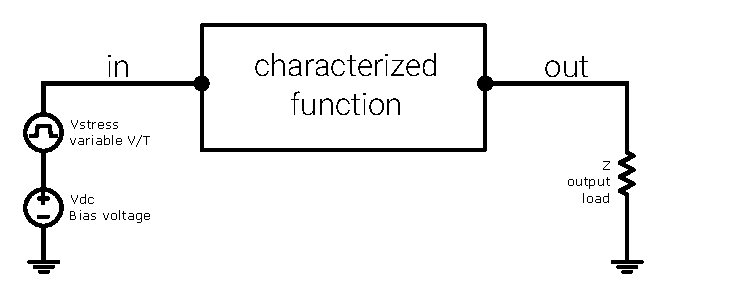
\includegraphics{src/1/figures/characterization_setup.pdf}
  \caption{Block characterization setup (supply input)}
  \label{block_function_cz}
\end{figure}

% What are the characterization signal
%TODO ref
Le signal de charactérisation est une impulsion rectangulaire, appliquée sur l'entrée sous test.
Un ensemble de simulations est effectué en faisant varier les paramètres de cette forme d'onde, injectée sur l'entrée.
Plus précisément, une analyse paramétrique est réalisée sur l'amplitude et la durée de l'impulsion.
Cet ensemble de simulations est résumé dans la Fig. \ref{set_input_signals}.
Cette méthode de charactérisation est fortement inspirée de la méthode Wunsch & Bell \cite{}.

%TODO: Fix sim 12 sim12
\begin{figure}[!h]
  \centering
  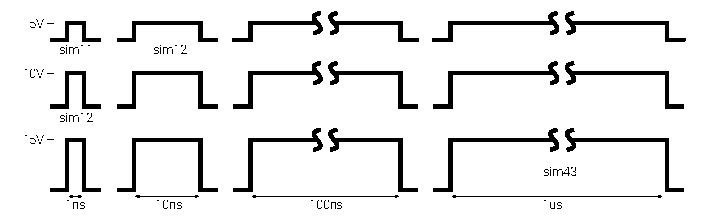
\includegraphics{src/1/figures/time_domain_cz_curves.pdf}
  \caption{Variations on (amplitude, duration) of the input characterization signal}
  \label{set_input_signals}
\end{figure}

Une fois chaque signal injecté, la sortie est observée.
Deux paramètres sont extraits de la forme d'onde de sortie.
L'amplitude maximale est extraite, correspondant à la plus large variation de tension par rapport à un niveau nominal.
La durée de cette variation, à 90\% de l'amplitude maximale est aussi relevée.
Ces deux paramètres permettent de décrire une boite englobante de la forme d'onde de sortie, constituant une sorte de forme d'onde simplifiée.
Cette analyse est effectuée pour chaque simulation.

Il en résulte deux tables, la première associant constituant le modèle du bloc.
La première table associes aux deux paramètres d'entrée (amplitude et durée) une amplitude maximale de sortie.
La seconde table associe aux deux paramètres d'entrée une durée de sortie.
Ces deux tables peuvent ensuite être intégrées dans un modèle, décrit Fig. \ref{fig:principle-transfert-func-v2}.
La fonction $F_{W}$ utilises la première table, pour retourner une amplitude de sortie en fonction des paramètres d'entrée.
La fonction $F_{V}$ utilises la seconde table et retourne une durée.
Sachant que ce modèle accepte les mêmes types de paramètres en entrée et en sortie, plusieurs modèles peuvent être chaînés les uns à la suite des autres, afin de reconstituer le comportement d'une fonction haut-niveau.

\begin{figure}[!h]
  \centering
  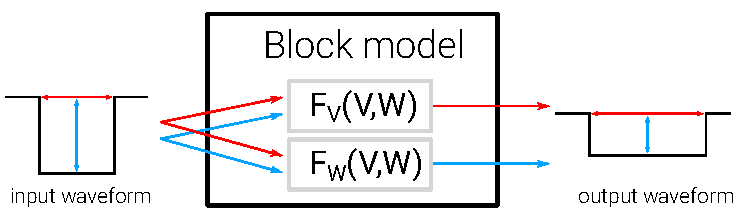
\includegraphics{src/1/figures/principle_transfert_function_v2.pdf}
  \caption{Improved modelling method}
  \label{fig:principle-transfert-func-v2}
\end{figure}

% First run the reference sim
Pour tester cette approche, des simulations sont effectuées en utilisant les schémas Fig. \ref{fig:hypothesis-setup}.
L'objectif est de comparer une simulation transistor de la fonction globale, à une chaine de simulation individuelle de blocs, pour vérifier si des réponses similaires peuvent être obtenues sur la broche de sortie lorsque la broche d'entrée est exposée au même stimuli.

\begin{figure}[!h]
  \centering
  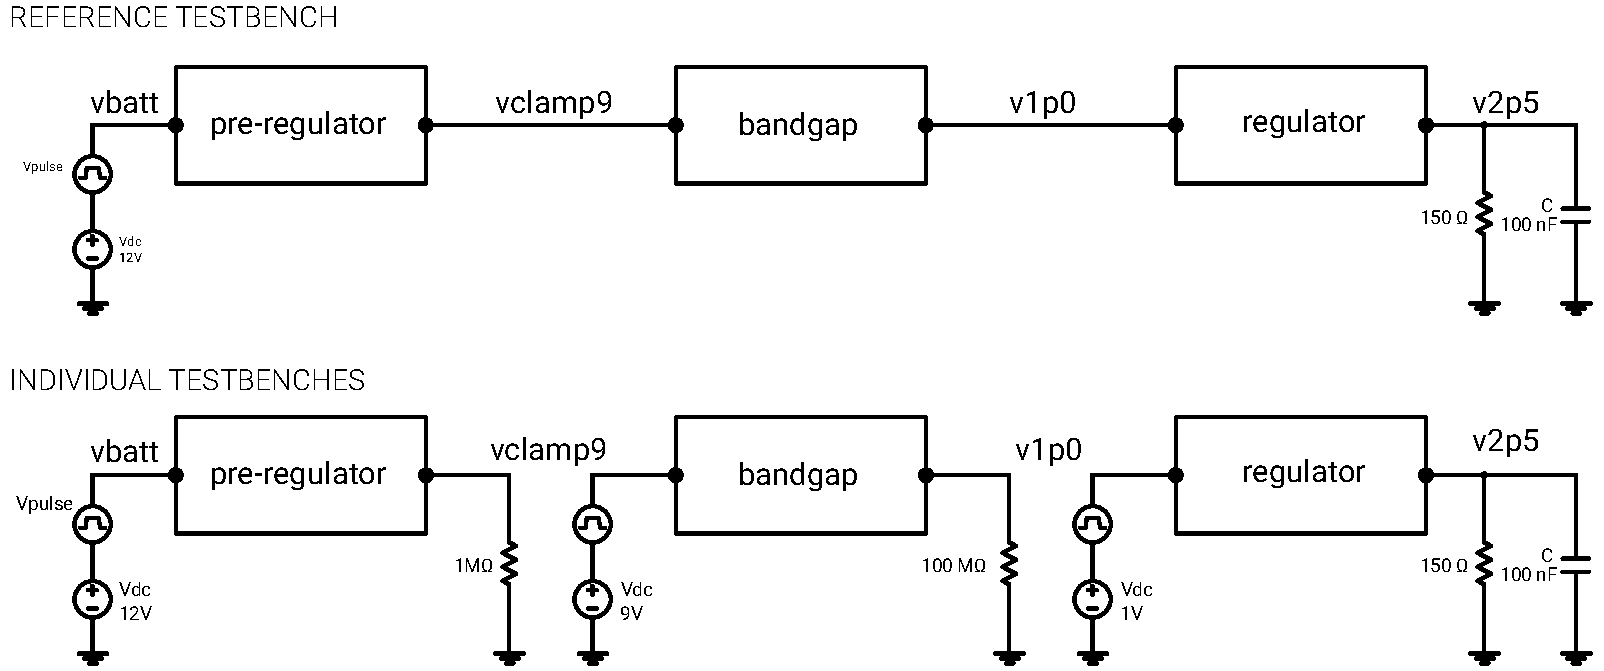
\includegraphics[width=0.98\textwidth]{src/1/figures/hypothesis_testing_setup.pdf}
  \caption{Testbenches used for characterization and hypothesis testing}
  \label{fig:hypothesis-setup}
\end{figure}

% Then do the same thing but with the individual models
La courbe du pré-régulateur seul est donnée Fig. \ref{fig:sim-compare-block1} et comparée avec la simulation totale.
Les deux courbes sont plutôt similaires.
La sortie est estimée avoir une amplitude maximale de -1.5 V (les stress sont d'amplitude négative) et une durée de 880 ns.
Ces deux valeurs sont utilisées comme paramètres d'entrée sur le second modèle, celui du bandgap.

\begin{figure}[!h]
  \centering
  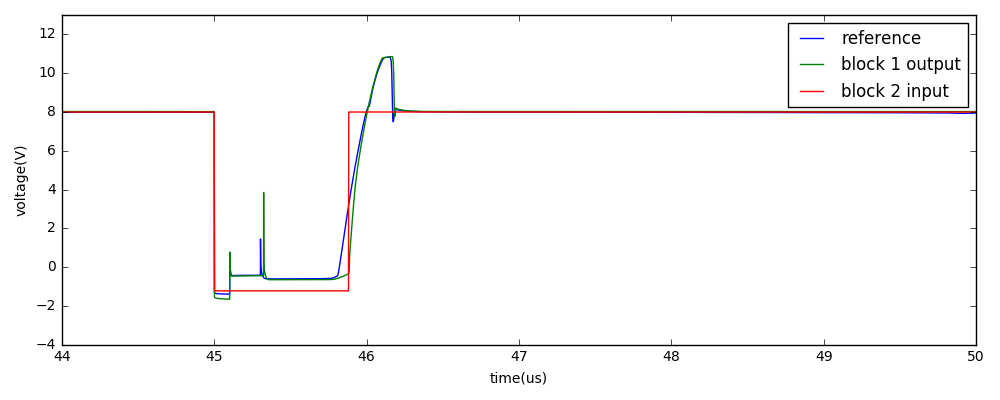
\includegraphics[width=0.98\textwidth]{src/1/figures/simulation_comparison_block1.png}
  \caption{$V_{clamp9}$ waveform}
  \label{fig:sim-compare-block1}
\end{figure}

% Second block output
A la sortie du second block, des différences plus larges apparaissent entre la simulation individuelle et totale. (Fig. \ref{fig:sim-compare-block2}).
La courbe verte a une pente plus longue que la référence.
Néanmoins, les courbes ont quand même des charactéristiques communes en terme d'amplitude maximale et de durée, ce qui est intéressant en regard de cette méthode de modélisation.
La courbe de sortie est analysée et son amplitude maximale déterminée à 0V avec une durée de 2 \textmugreek{}s.
Ces deux valeurs sont appliquées sur l'entrée de la troisième simulation.

\begin{figure}[!h]
  \centering
  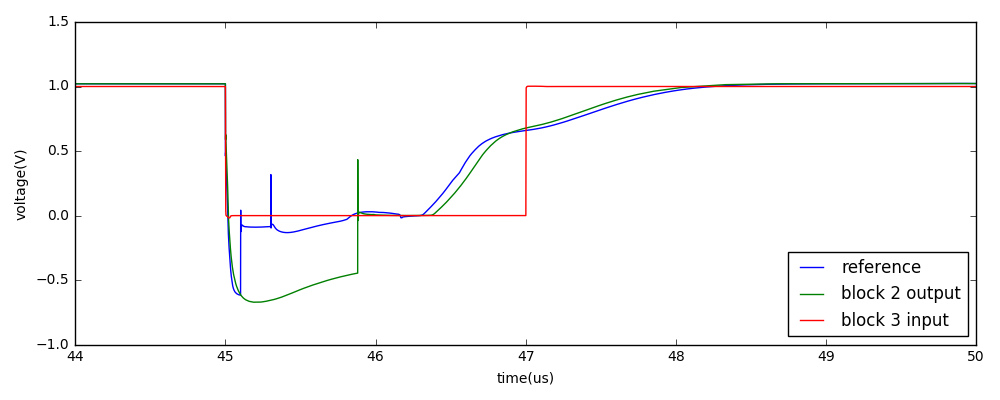
\includegraphics[width=0.98\textwidth]{src/1/figures/simulation_comparison_block2.png}
  \caption{$V_{1p0}$ waveform}
  \label{fig:sim-compare-block2}
\end{figure}

% Third output
A la sortie du dernier bloc, (Fig. \ref{fig:sim-compare-block3}), les deux formes d'onde sont similaires.
La différence d'amplitude maximale est due à un offset aussi présent en statique, et pouvant donc être aisément corrigé.
La courbe de référence est retardée par rapport à la courbe individuelle, mais sinon les deux courbes se ressemblent énormément.

\begin{figure}[!h]
  \centering
  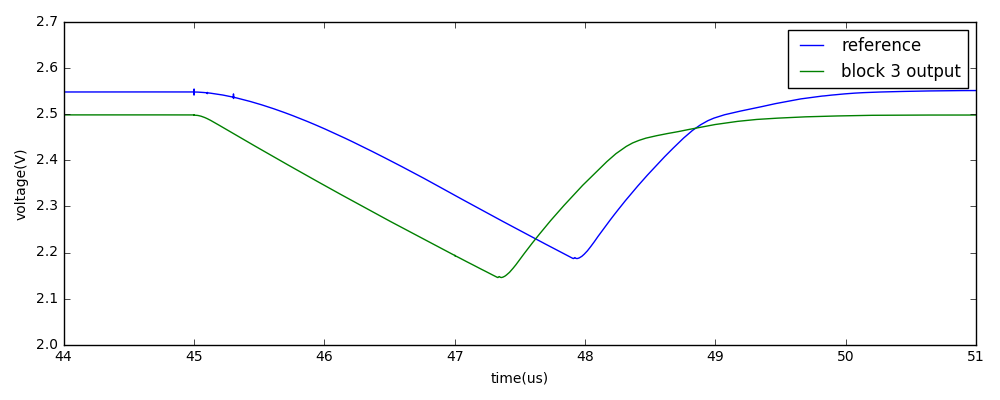
\includegraphics[width=0.98\textwidth]{src/1/figures/simulation_comparison_block3.png}
  \caption{$V_{2p5}$ waveform}
  \label{fig:sim-compare-block3}
\end{figure}

% Conclusion, it works for this case
En conclusion, pour ce cas d'étude, la méthode de simulation et modélisation individuelle aurait permit, par chainage des modèles d'estimer correctement la perturbation sur le bloc de sortie.
Avant de pouvoir généraliser son utilisation, il serait nécessaire de tester cette méthode sur une plus large gamme d'applications.
Elle montre néanmoins des résultats prometteurs.

\section{Méthode boite noire}

% Difference with bottom-up, not the same application, not the same goal
The black-box modeling method relies on the same core principles than the bottom-up modeling approach.
It studies the relationship and transfert function between the input and the output of a silicon function.
Unlike the bottom-up method though, the model is only built for external input and output pins.
It is not meant to be chained with other models, using a special chaining method.
Instead, it targets electrical, board-level circuit simulations.
Basically, the black box model is intented to act as a drop-in replacement for the complete \gls{ic} circuit, for board-level simulations.

% introduction, failure relation between input and output
The main benefit of this model is to abstract the internal silicon complexity.
The model focuses on describing the failure of an output when an input is stressed.
At board-level, failure criteria can be more easily set from the chip specification.
After setting the failure criteria, the approach is to inject rectangular pulses on an input pin, and record when an output is in fault.


% How is the characterization conducted
Once again, a variable width/variable amplitude rectangular pulses are applied on an input pin.
The output pin is then observed to detect for which input parameters it is going out of specification.

% What is characterized
This characterization is performed on the testchip, on the complete regulation function.
The characterization pulses are injected on the $V_{batt}$ input.
The output pin is $V_{2p5}$, the regulated supply.
It is supposed to deliver a 2.5V regulated supply.
The failure criteria is set at a voltage below 2.1V.
It corresponds to a level below which digital cells powered by this supply will have noise margins too small for proper operation.

% Fig X shows the waveform of the VBAT injected current when stressed with a TLP (square) impulse.
% The TLP waveform before the capacitor is shown for reference.
%TODO: WAVEFORM CURRENT VBAT AND TLP BEFORE INJECTION CAPACITOR ?

% Detail the characterization
The characterization table is plotted in Fig. \ref{fig:cz-black-box}.
X-axis is the pulse width, and y-axis is the minimal stress amplitude that caused a failure on the output.

\begin{figure}[!h]
  \centering
  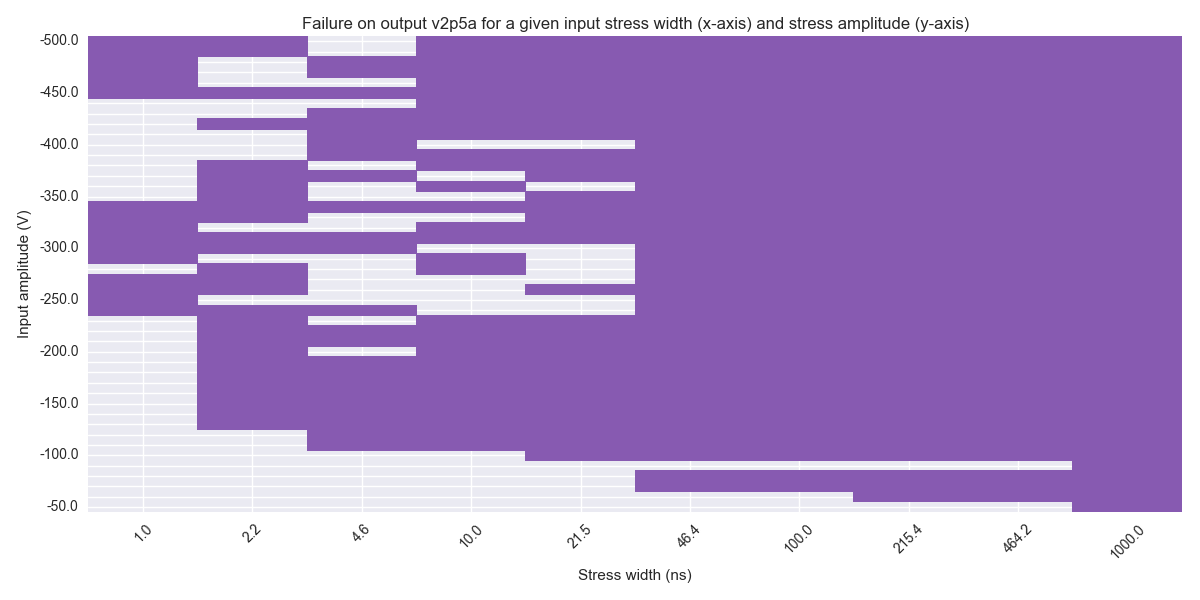
\includegraphics[width=\textwidth]{src/1/figures/black_box_regulator.png}
  \caption{Black-box characterization of the regulation function}
  \label{fig:cz-black-box}
\end{figure}

% What to do with that
%TODO: We that below this value the function is in fail, etc
However, the motivation for this model is to replace the transistor-level schematic inside a SPICE simulation at board-level.
Given a pulse width and an amplitude on $V_{batt}$, the model can estimate the disturbance amplitude and width on $V_{2p5}$.
However, the model itself is not an electrical model, only a failure model.
It cannot determinate, given for instance an input voltage, how much current is flowing into it.
This is also true for the output.
Thus, this method calls for an electrical model of \gls{io}.

\gls{tlp} characterizations are performed on the testchip's regulation function, in powered and unpowered conditions.
For powered conditions, it is considered that full functionality and performance does not matter, just the equivalent impedance of the input or output.
As a consequence, the function is biased but external devices are not connected.
Unpowered and powered characterizations are compared respectively in Fig. \ref{fig:tlp-input-cz} and \ref{fig:tlp-output-cz}.

\begin{figure}[!h]
  \centering
  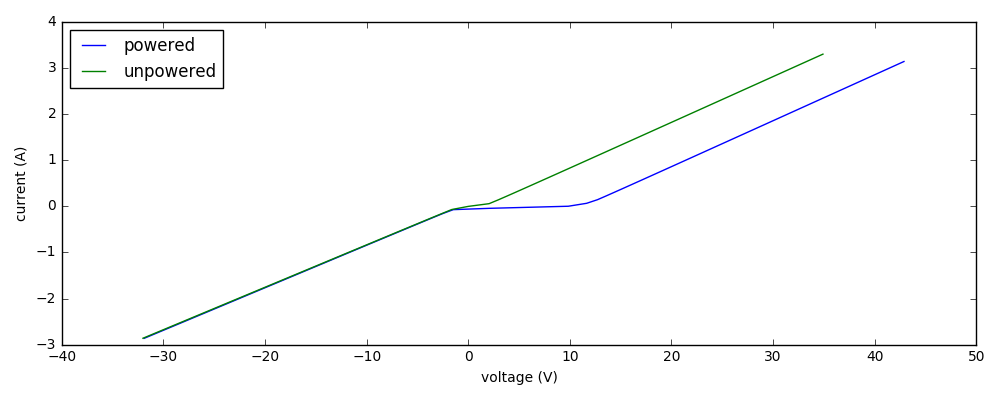
\includegraphics[width=\textwidth]{src/1/figures/tlp_input_characterization.png}
  \caption{TLP characterization of function input in powered and unpowered conditions}
  \label{fig:tlp-input-cz}
\end{figure}

\begin{figure}[!h]
  \centering
  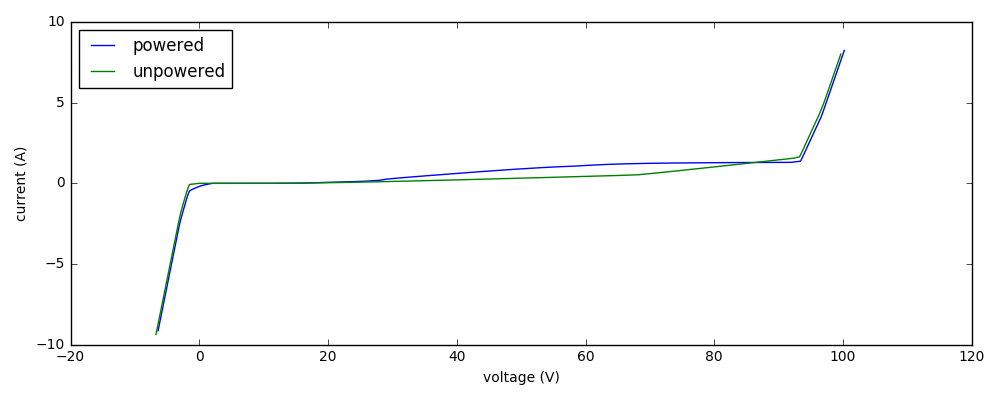
\includegraphics[width=\textwidth]{src/1/figures/tlp_output_characterization.png}
  \caption{TLP characterization of function output in powered and unpowered conditions}
  \label{fig:tlp-output-cz}
\end{figure}


For both input and output ports, large differences are observed between powered and unpowered modes.
Different amount of current are absorbed by the device in each conditions.
Since the model is intended for powered-on simulations, the characterization in powered conditions is chosen.

% Explain the PWL model
The second step of the modelling method is to build an electrically simulatable model of the function.
A piecewise linear model seems well suited for this situation.


% Validate the model with TLP
The verilog-a model is first tested against the complete schematic for the function's input.
After issues described previously were solved, good agreement is achieved between model and complete circuit.
This was verified at -10V, 20V and 40V TLP amplitude (Fig. \ref{fig:compare-model-simu-m10}, Fig. \ref{fig:compare-model-simu-20}, Fig. \ref{fig:compare-model-simu-40}).
The model is considered mostly valid for the input.

\begin{figure}[!h]
  \centering
  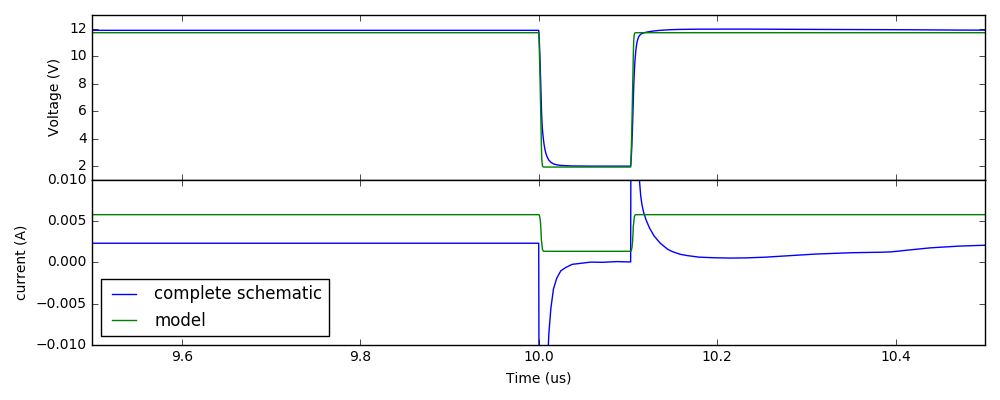
\includegraphics[width=\textwidth]{src/1/figures/comparison_model_total_m10V.png}
  \caption{Comparison of complete schematic and model simulations - -10V TLP}
  \label{fig:compare-model-simu-m10}
\end{figure}


% Check the output
The same test is performed for the function's output model.
The situation is more complex in this case.
The output model must perform three tasks.
First, offer an output impedance close the the one of the real function.
Second, provide a DC value, here corresponding to the regulated 2.5V.
Lastly, reproduce the function reset where the output voltage falls down then restarts.
A first output model is envisionned (Fig. \ref{fig:first-output-model}).

\begin{figure}[!h]
  \centering
  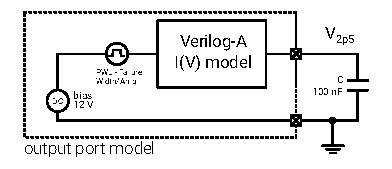
\includegraphics[width=0.3\textwidth]{src/1/figures/first_output_model.png}
  \caption{First proposal for modeling function output}
  \label{fig:first-output-model}
\end{figure}

% Is this first model working
Preliminary and extended tests show that this configuration is not working.

%TODO: Du coup on fait quoi ?


% Conclusion
Black box models of analog integrated functions are very interesting for distributing SPICE models to external parties.
They do not disclose the internal design of the chip, yet they can help achieve system-level ESD simulations.
Ultimately, the goal is to follow the SEED (TODO: Ref) methodology, that indicates that ESD robustness should not be handled at a single level of a system, but at every level (equipment, board, integrated circuit), and that all levels should work efficiently together toward that goal.
Black box models fit very nicely in this methodology.
In this section, a first technique for extracting and creating black-box models was presented.
There is a lot of room for improvements, but it is already working for some intermediate complex cases.
The core principle is that TLP characterization of inputs and ouputs on a biased function is sufficient to extract an equivalent impedance.
This impedance can replace the function in the schematic, during an ESD simulation, in order to reduce complexity and simulation time.
The second core principle is to simplify waveforms into rectangular ones in order to reduce the complexity of the problem.

% Opening work
There are many new leads to explore on these black box models.
First, behavior of the models against more time-varying disturbances such as ESD gun waveforms should be investigated.
Also, the piecewise-linear models should be improved to be more stable, and to fit more closely the extracted I(V) curve.
This technique should be applied to a wider number of analog functions, to observe if it can be used in a general manner.
For now, input and outputs must be simulated separately.
First, the input is simulated, then analyzed to extract the width and amplitude of the disturbance.
This data is then used to configure the output failure source pulse.
The model must be improved in order for the output to react in real-time to the disturbance of the input.
Ultimately, this calls for a Verilog-A model of the failure for instance, plus most likely an improved characterization method able to extract and describe this real-time behavior.
